\documentclass[12pt, a4paper]{scrartcl}
\usepackage[utf8]{inputenc}
\usepackage[T1]{fontenc}
\usepackage[ngerman]{babel}
\usepackage{SIunits}
\usepackage{graphicx}
\usepackage{amsmath}
\usepackage{enumitem}
\usepackage{float}
\usepackage{verbatim} %für Kommentare
\usepackage{listings} %Zur Code-Einfügung
 \usepackage{subfigure}  %Bilder nebeneinander darstellbar

\usepackage[
colorlinks,
pdfpagelabels,
bookmarksopen = true,
bookmarksnumbered = true,
linkcolor = black,
plainpages = false,
hypertexnames = false,
citecolor = black
]{hyperref}

\usepackage[subfigure]{tocloft}
%Punktlinie auch nach Kapiteln im Inhaltsverzeichnis
\renewcommand{\cftsecleader}{\cftdotfill{\cftdotsep}}

%Zeilenabstände
\renewcommand{\baselinestretch}{1.5} 

\usepackage{geometry}
%Rand-Abstände
\geometry{verbose, left=20mm, right=20mm, top=30mm, bottom=30mm}

%\usepackage{titlesec}
%\titleformat
%{\chapter} % command
%[hang] % shape
%{\bfseries\Huge} % format
%{\thechapter} % label
%{0.5ex} % sep
%{} % before-code
%[] % after-code


% Für Grafiken
\usepackage{tikz}
\usepackage{pgfplots}


%%%%%%%%%%%%%%%%%%% Aufteilung: %%%%%%%%%%%%%%%%%%%
% Lea:
%Abstandserkennung
%(GeogebraDatei im doc Ordner)

% Adrian:
%Motoransteuerung
%Umgebung (Räumliche Umgebung des Autos mit Bildern. Auch aus der Sicht des Autos)

% Julian W.:
%Softwareplattform
%Interprozesskommunikation

% Julian F.
%Linienerkennung
%Zielsetzung

% René
%Hardwareplattform
%Einleitung
%Struktur

% Gemeinsam:
%Komplikation und Fehler
%Auswertung


\begin{document}

%%%%%%%%%%%%%%%%%%% STARTSEITE %%%%%%%%%%%%%%%%%%%

\begin{center}
	
	\begin{figure}[H]
		\centering
		
\includegraphics[width=10cm]{Bilder/fh-wedel-logo.png}
	\end{figure}

	\vspace*{1.5cm}
	\Large{\textbf{ R O B O T I K\quad P R A K T I K U M \\ Wintersemester 2017/ 2018\\}}
	\vspace*{1.5cm}
	\huge{\textbf{Dokumentation - Gruppe 1\\}}
	\vspace*{1.5cm}
	
	\vfill
	\begin{table}[h]\centering
		\begin{tabular}{l l}
			 &  tinf101030 - Julian Finck \\
			 & \\
			 & tinf101364 - René P. Keller  \\
			 & \\
			 & inf101301 - Lea Morschel \\
			 & \\
			 & tinf101313 - Adrian Sorge \\
			 & \\
			 & tinf101087 - Julian Weihe \\
		\end{tabular}
	\end{table}

\end{center}

\thispagestyle{empty} %keine Seitennummer auf Startseite

\newpage
\tableofcontents % generiertes Inhaltsverzeichnis
\thispagestyle{empty} %keine Seitennummer beim Inhalsverzeichnis
\newpage
\pagenumbering{arabic}


%%%%%%%%%%%%%%%%%%% INHALTE %%%%%%%%%%%%%%%%%%%

%%% Neues Kapitel %%%
\section{Einführung}

Das Robotik-Praktikum, dessen Ergebnis diese Dokumentation festhält, findet parallel und in Kombination mit der Bachelor-Vorlesung 'Einführung in die Robotik' statt, welche von Herrn Prof. Dr. Ulrich Hoffmann im Wintersemester 2017 gehalten wird.

Ziel ist die Vertiefung und Anwendung der in der Vorlesung vermittelten Inhalte, wobei der diessemestrige Schwerpunkt  auf autonomen Robotern liegt. Im Praktikum, unter der Leitung von Hermann Höhne, wird mit einem AADC\footnote{Audi Autonomous Driving Cup: \url{https://www.audi-autonomous-driving-cup.com/wettbewerb/ueberblick/}} 2017 Audi-Modell im Maßstab 1:8 gearbeitet. Es soll zu Beginn eine nicht näher eingeschränkte Zielsetzung ausgearbeitet werden, welche auf der grundlegenden Anforderung der kollisionsfreien Fahrt aufbaut.

%%% Neues Kapitel %%%
\subsection{Zielsetzung} \label{zielsetzung}

Im Kontext der gegebenen Grundanforderung der Kollisionsvermeidung werden eigene Ziele definiert. Das Auto soll später in der Lage sein, unter verschiedenen Lichtverhältnissen, einer zentralen blauen Fahrbahnmarkierung zu folgen. Bei Näherkommen eines von Ultraschallsensoren detektierbaren Hindernisses soll das Modell langsamer werden und vor ihm zum Stehen kommen sowie die Fahrt erst wieder aufnehmen, wenn die Sensoren signalisieren, dass die Fahrbahn wieder frei ist.

Die zu Beginn des Praktikums ausgearbeitete Roadmap findet sich in Abbildung \ref{img:Roadmap_Gr1}.
\newpage
Die Umsetzung des Projektes wird zu Anfang in vier Bereiche unterteilt:
\begin{enumerate}
		\item{Linienerkennung und -verwertung
		\begin{enumerate}
			\item Mittelpunktbestimmung
			\item Testen unter verschiedenen Lichtintensitäten
	\end{enumerate}}
	\item{Abstandserkennung und Kollisionsvermeidung
	\begin{enumerate}
		\item Messwertverarbeitung der Ultraschallsensoren
		\item Messwertglättung durch Filterung (Kalman)
	\end{enumerate}}
	\item {Motorsteuerung
		\begin{enumerate}
		\item Schnittstellendefinition zur Ansteuerung
		\item Steuerung von Geschwindigkeit und Lenkung
		\end{enumerate}}
		\item{Zusammenbringung/ Fusionsschnittstelle
		\begin{enumerate}
			\item Definition und Ausarbeitung des Controllers (Verhaltens-Logik)
			\item Problembehandlung, Feinabstimmung, Testung
		\end{enumerate}}
\end{enumerate}

\begin{figure}
\centering
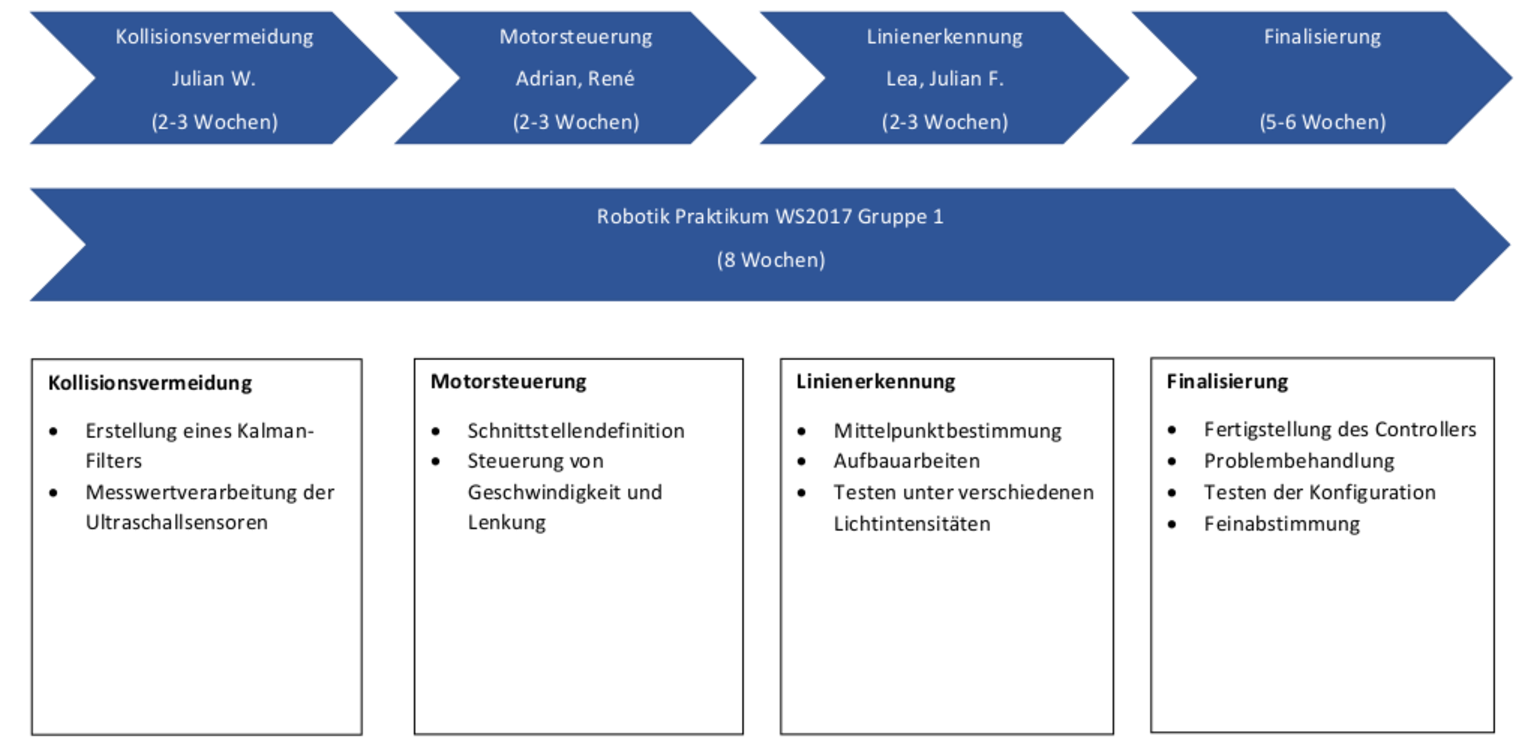
\includegraphics[width=\textwidth, height=9cm, keepaspectratio]{Bilder/Roadmap_Gr1.pdf}
\caption{Zu Projektbeginn erstellte Roadmap}
\label{img:Roadmap_Gr1}
\end{figure}


\newpage
%%% Neues Kapitel %%%
\section{Grundlagen}
Im Folgenden werden die Grundlagen, bestehend aus Aufbau des genutzten Modellautos, der darauf laufenden Software sowie das genutzte Framework erläutert, welche für das Verständnis des Projektes essenziell sind.

\subsection{Hardwareplattform}
Das Audimodell bietet verschiedene Hardwarekomponenten, um das autonome Fahren zu verwirklichen. Es ist in \autoref{img:carSide_table} zu sehen.

\begin{figure}[ht]
	\centering
	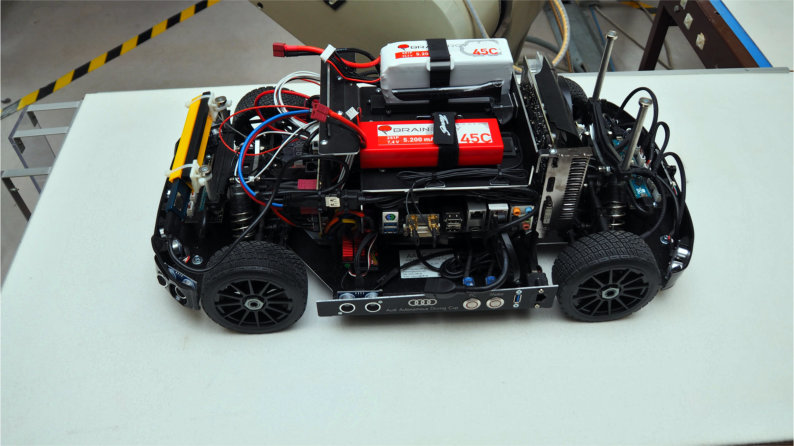
\includegraphics[width=0.9\textwidth, keepaspectratio]{Bilder/carSide_table.jpg}
	\caption{Seitliche Ansicht des im Projekt verwendeten Audi-Modells}
	\label{img:carSide_table}
\end{figure}

\subsubsection{Grundkomponenten}
Die Stromversorgung der Steuerung und der Motoren während der Fahrt wird jeweils von einem separaten Akku gewährleistet.

\subsubsection{Rechner}
Herzstück des Audi ist das \emph{GIGABYTE GA-Z170N-WIFI miniITX} Mainboard mit einem \emph{Intel Core i3-6100T} und 8 GB DDR4 RAM. Unterstützt wird es von einer \emph{NVIDIA GeForce GTX 1050Ti}.

Das Betriebssystem wird von einem USB-Stick gebootet, um das Auto mit mehreren Gruppen nutzen zu können.

\subsubsection{Aktoren}
Angetrieben wird das Modell von einem \emph{Hacker SKALAR 10 21.5 Brushless Motor 1/10}.
Die Lenkung funktioniert über einen \emph{Absima 'ACS1615SG' Combat Series} Servo. 

\subsubsection{Sensoren}
Eine visuelle Erfassung der Umwelt erfolgt durch eine frontal angebrachte Tiefen-Kamera und eine rückwärtige RGB-Kamera. Zur Abstandsdetektion sind 10, in verschiedene Richtungen schauende Ultraschallsensoren angebracht (siehe \autoref{img:car_ussensors}). Beschleunigung, Ausrichtung und Lage im Raum werden vom einem Motion-Tracking Sensor übernommen. Aufschluss über die Radstellung wird mittels Drehgeber gegeben. Das Auslesen der Sensordaten erfolgt über Arduinos, welche per USB Protokoll die Daten zum Mainboard senden.

\begin{figure}[ht]
	\centering
	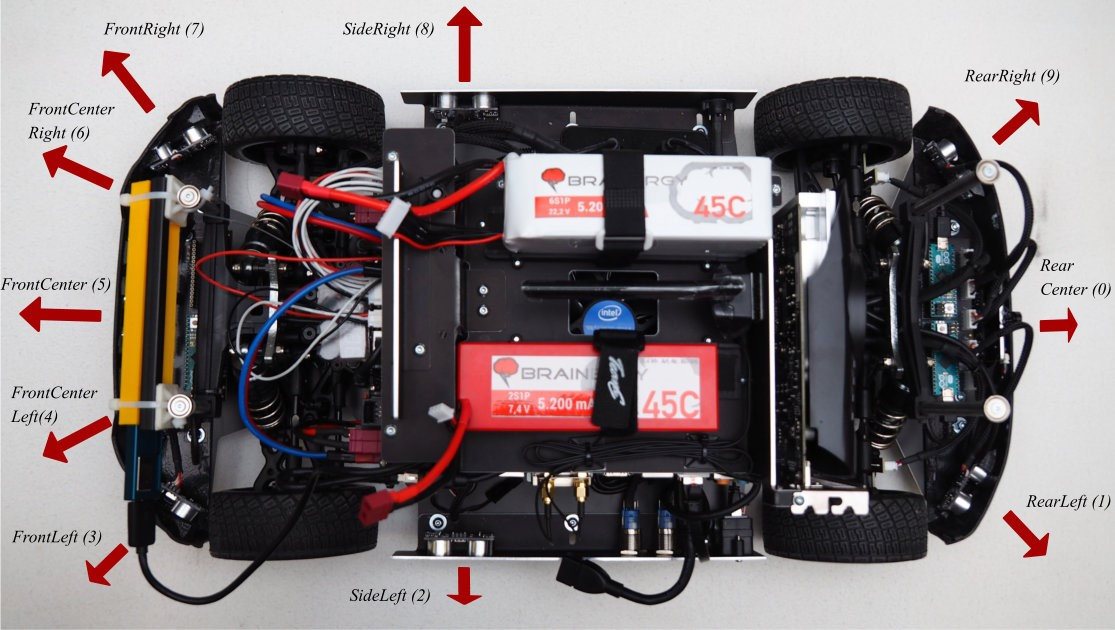
\includegraphics[width=\textwidth, height=10cm, keepaspectratio]{Bilder/car_sensors.jpg}
	\caption{Platzierung der Ultraschallsensoren am Audi-Modell}
	\label{img:car_ussensors}
\end{figure}

\begin{comment}
\begin{figure}[ht]
	\centering
	\begin{tikzpicture}[xscale=0.05,yscale=0.05]
	
	%Auto-Umriss
	\draw[line width=0.2mm] (-20,20) -- (-10,0) -- (10,-10) -- (40,-10) -- (60,0) -- (70,20); %Hinterseite
	\draw[line width=0.2mm] (-20,120) -- (-20,20);	%linke Seite
	\draw[line width=0.2mm] (70,20) -- (70,120);	%rechte Seite
	\draw[line width=0.2mm] (-20,120) -- (-10,140) -- (10,150) -- (40,150) -- (60,140) -- (70,120); %Vorderseite
	
	\draw[line width=0.2mm, ->] (25,50) -- (25,100); %Mittelpfeil
	
	%Pfeile und Beschriftungen der Sensor-Lagen
	\draw[->] (50,0) -- (60,-15) node[below right]{$Rear Right(9)$};
	\draw[->] (65,70)-- (80,70) node[right]{$Side Right(8)$};
	\draw[->] (60,130) -- (80,140)  node[above right] {$Front Right(7)$};
	\draw[->] (45,140) -- (65,160)  node[above right] {$Front Center Right(6)$};
	\draw[->] (25,145) -- (25,170) node[above] {$Front Center(5)$};
	\draw[->] (5,140) -- (-15,160)  node[above left] {$Front Center Left(4)$};
	\draw[->] (-10,130) -- (-30,140)  node[above left] {$Front Left(3)$};
	\draw[->] (-15,70) -- (-30,70) node[left]{$Side Left(2)$};
	\draw[->] (0,0) -- (-10,-15) node[below left]{$Rear Left(1)$};
	\draw[->] (25,-5) -- (25,-20) node[below]{$Rear Center(0)$};
	
	\end{tikzpicture}
	\caption{Platzierung der Ultraschallsensoren am schematischen Modell}
	\label{graph:us-car}
\end{figure}
\end{comment}

\subsection{Softwareplattform}
Das Modellauto verwendet die Ubuntu Version 16.04 und zur Bildschirmübertragung ist der x11vcn Serverdienst eingerichtet. Die Software EB Assist ADTF 2.14 von Elektrobit ist installiert, um die damit bereitgestellte Programmoberfläche und das ADTF-Framework\footnote{Automotive Data and Time-Triggered Framework: \url{https://www.elektrobit.com/products/eb-assist/adtf/}} zu verwenden.

\subsubsection{ADTF-Framework: Grundlegende Strukturen}
 Das Framework stellt Funktionen zur Kommunikation mit den im Abschnitt 'Hardwareplattform' erläuterten Sensoren und Kameras bereit. Außerdem ermöglicht es eine Programmaufteilung in Funktionsblöcke, \emph{Filter} genannt, welche parallel auf mehreren Prozessorkernen ausgeführt werden können. Die Kommunikation zwischen diesen Blöcken wird über Nachrichtenqueues und Priorisierung vom Framework sichergestellt. Die Ausführung der Funktionsblöcke wird einstellbar, periodisch und eventgesteuert ausgelöst und beginnt meist mit dem Anstoß zum Auslesen der Sensoren, welche dann das Event über die Queues an andere Funktionsblöcke weitergeben.

Von der Benutzeroberfläche aus lassen sich die Funktionsblöcke grafisch miteinander verbinden, welches die Kommunikation zwischen den Blöcken repräsentiert, und die Ausführung der Funktionen starten. Des Weiteren gewährt die Oberfläche Zugriff auf fertige Funktionsblöcke, etwa zum Anzeigen und Abspeichern von Kamerabildern und Sensordaten oder zum  Abspielen selbiger.
Durch Referenzen aus dem Programm heraus können über die Benutzeroberfläche bestimmte Parameter zur Initialisierung und zur Laufzeit gesetzt werden.


\newpage
%%% Neues Kapitel %%%
\section{Implementierung}

\subsection{Umgebung}

Die Zielsetzung sieht vor, das Auto eine blaue Linie verfolgen zu lassen. Zu Testzwecken wird daher auf dem hell grauen Boden eine große, ovalförmige Linienstruktur mit mattblauem Klebeband befestigt, deren Maße etwa 1,5 m x 3 m beträgt. Zur Vermeidung von störender Spiegelung wird zudem das Fenster zugestellt, um die Sonneneinstrahlung zu minimieren.

\subsection{Projektumsetzung}

Das Projekt wird zu Beginn in drei verschiedene Aufgabenbereiche aufgeteilt, die separat bearbeitet werden (siehe \autoref{zielsetzung}). Diese werden im Folgenden näher beschrieben.

\begin{enumerate}
	\item Linienerkennung und -verfolgung
	\item Abstandserkennung und -verwertung
	\item Motorsteuerung
\end{enumerate}

\subsubsection{Linienerkennung und -verfolgung}
Damit das Auto der blauen Fahrbahnlinie folgen kann, wird die Linie im Kamerabild detektiert. Anschließend wird die Position der Linie ausgewertet, um daraus Steuersignale für die Lenkung zu gewinnen. Diese Aufgaben werden von zwei Filtern gelöst:

\paragraph{BlueImgFilter}
\begin{figure}[h]
	\centering
	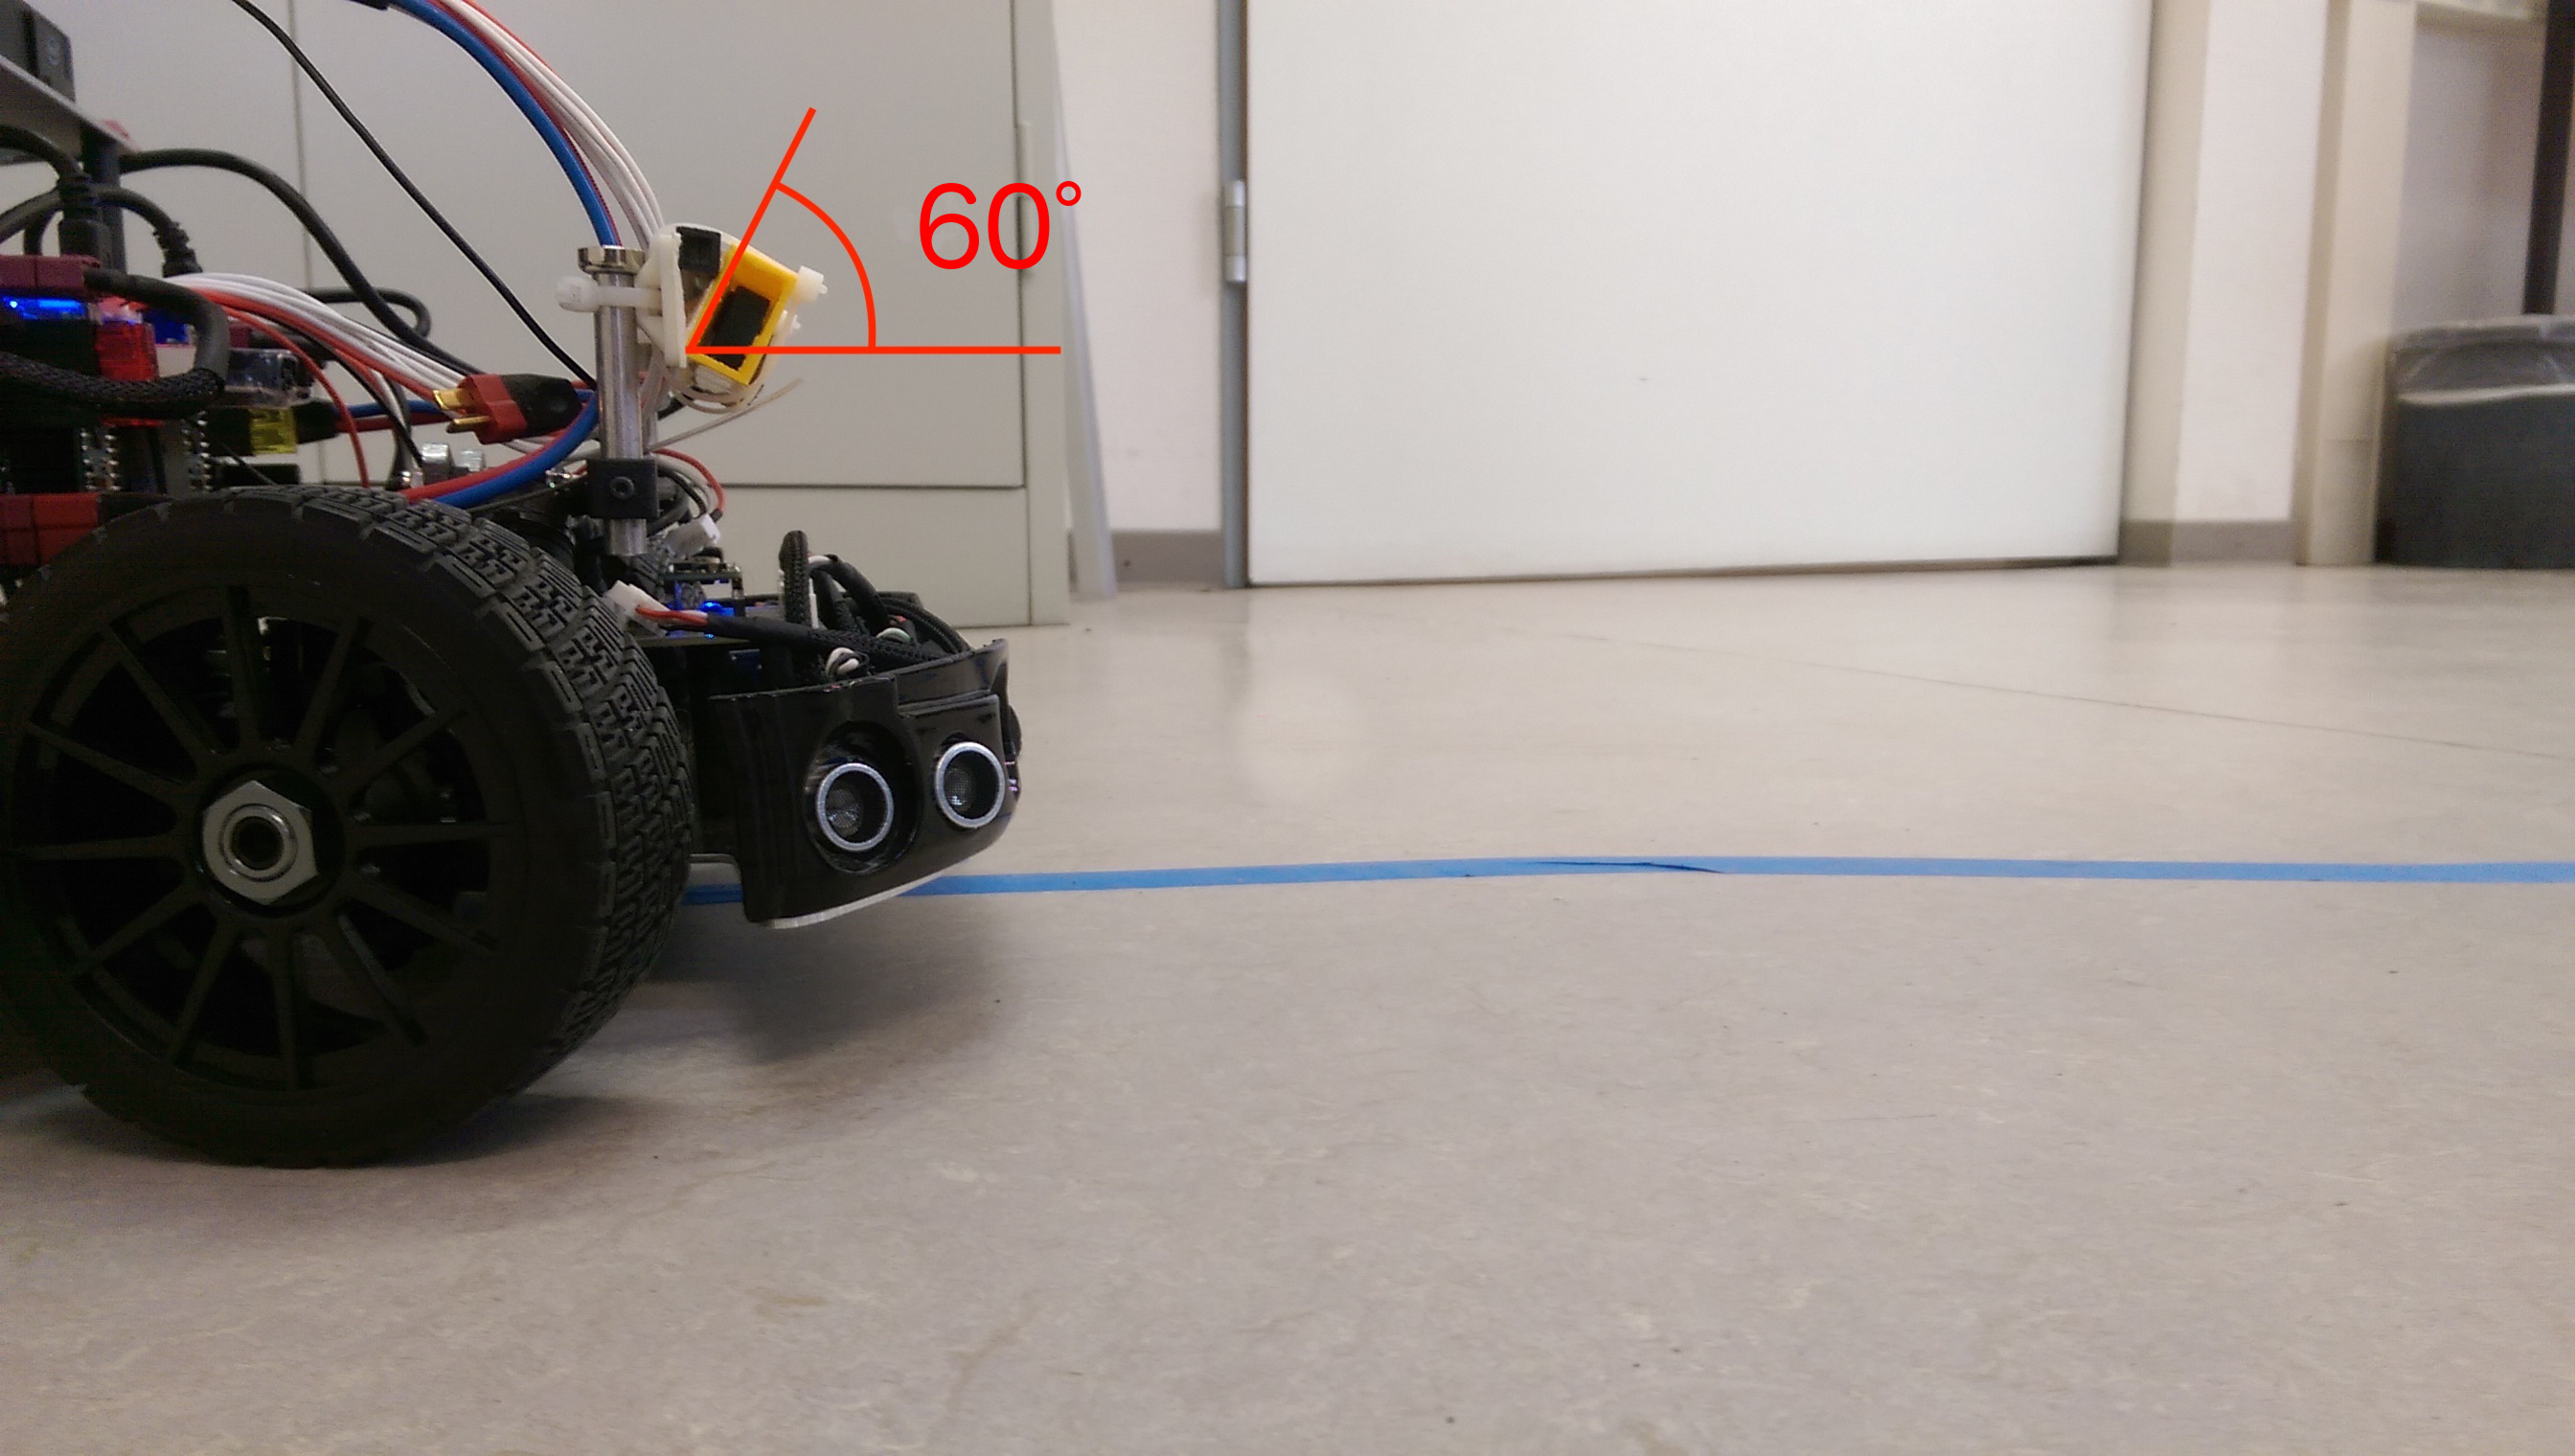
\includegraphics[width=\textwidth, height=7cm, keepaspectratio]{Bilder/carCameraFrontAngle60.jpg}
	\caption{Winkel der Frontkamera am Modell}
	\label{img:carCameraFrontAngle60}
\end{figure}

Dieser Filter markiert die Fahrbahnlinie und greift dafür auf die OpenCV Bibliothek zurück. Die Kamera ist in einem 60 Grad Winkel montiert (siehe \autoref{img:carCameraFrontAngle60}). Es ist davon auszugehen, dass die Fahrbahnlinie der einzig blaue Bildinhalt im relevanten Bildausschnitt ist. Zunächst wird das Eingangsbild mit OpenCV vom RGB- in den HSV-Farbraum transformiert, um die Festlegung des Farbbereiches für Blauwerte zu vereinfachen. Mittels der OpenCV-Funktion \emph{inRange()} werden anschließend alle nicht blauen Bildinhalte heraus gefiltert und ein Binärbild zurückgegeben, welches alle blauen Flächen markiert. Die endgültigen Farbwertgrenzen sind das Ergebnis von folgenden Versuchen mit variierenden Lichtverhältnissen:

\begin{description}
	\item[Versuch 1 - Szenario mit geringster Lichtintensität]
	Lichtverhältnisse:	Jalousie runter gelassen, Beleuchtung aus, Tageslicht von den Oberlichtern, bewölkt (mittags)
	\item[Versuch 2 - Szenario mit höchster Lichtintensität]
	Lichtverhältnisse:	Jalousie oben, alle Lichter an, keine Wolken (mittags) 
\end{description}

Auswertung:

Als Ergebnis dieser Versuche sind die in \autoref{tbl:linedet_lighttest} folgenden Unter- bzw. Obergrenzen der Funktion \emph{inRange()} eruiert worden, welche in beiden Extremfällen eine Positionsberechnung der Linie ermöglichen.

\begin{table}[h]
	\caption{Ergebnisse der Tests bei verschiedener Lichtintensität}
	\centering
	\begin{tabular}{ c | c | c |}
		& Untergrenze & Obergrenze \\ \hline
		Hue & 95 & 130 \\ \hline
		Saturation & 100 & 255 \\ \hline
		Value & 70 & 255 \\
	\end{tabular}
	\label{tbl:linedet_lighttest}
\end{table}

Im dunklen Szenario beeinträchtigt der geringe Rauschabstand die Erkennung der Linie leicht, wie in \autoref{img:line_filt_viel_u_wenig_licht} (b) zu erkennen ist. Die Ergebnisse lassen dennoch eine ausreichend robuste Positionsberechnung zu.

Im hellen Szenario ist der Rauschabstand so groß, dass \emph{inRange()} die Fahrbahnmarkierung nahezu optimal ausschneidet (\autoref{img:line_filt_normal_u_kurve} (a)). Reflexionen der Sonne können zu Clipping führen und verhindern eine durchgehende Erkennung der Markierung (siehe \autoref{img:line_filt_viel_u_wenig_licht} (b)).

\begin{figure}[h]
	\subfigure[Viel Licht und Reflektion]{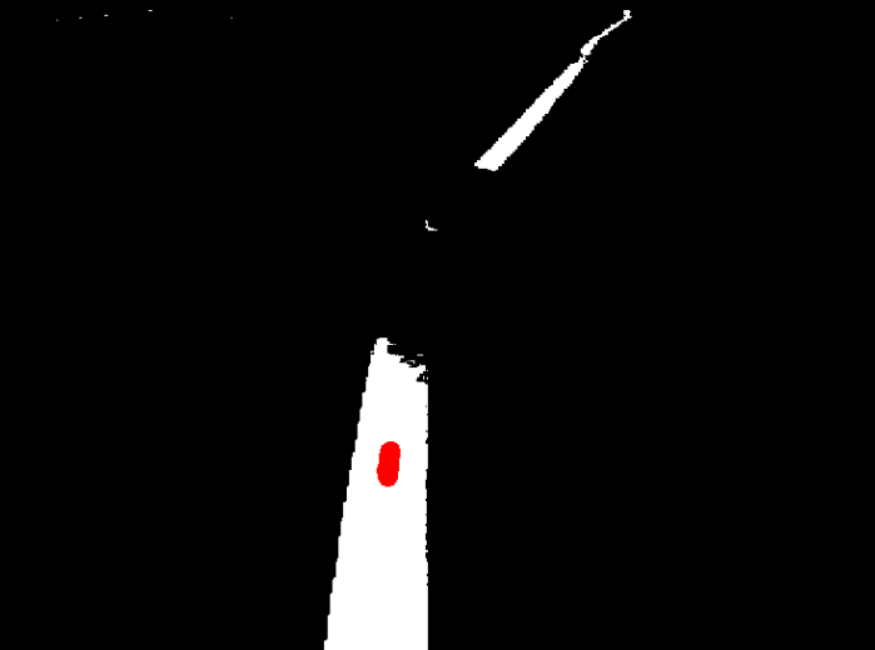
\includegraphics[width=0.49\textwidth]{Bilder/line_filt_vielLicht_reflektion.png}}
	\subfigure[Wenig Licht]{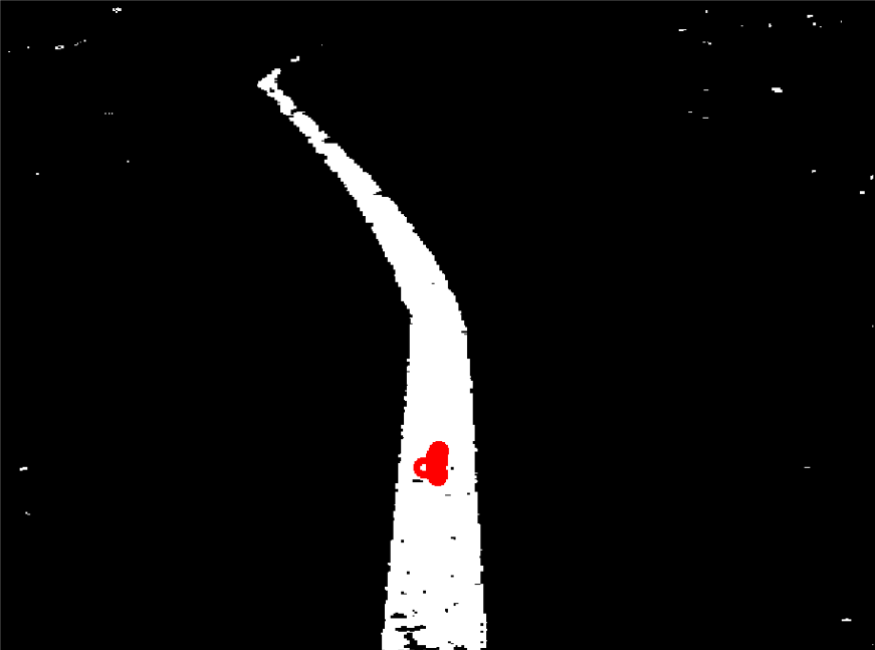
\includegraphics[width=0.49\textwidth]{Bilder/line_filt_wenigLicht.png}}
	\caption{Gefilterte Linienerkennung unter extremen Lichtverhältnissen}
	\label{img:line_filt_viel_u_wenig_licht}
\end{figure}

Daher ist es wichtig, direkte Sonneneinstrahlung auf der Fahrbahn zu vermeiden.  

\begin{comment}
	\begin{figure}[h]
	\centering
	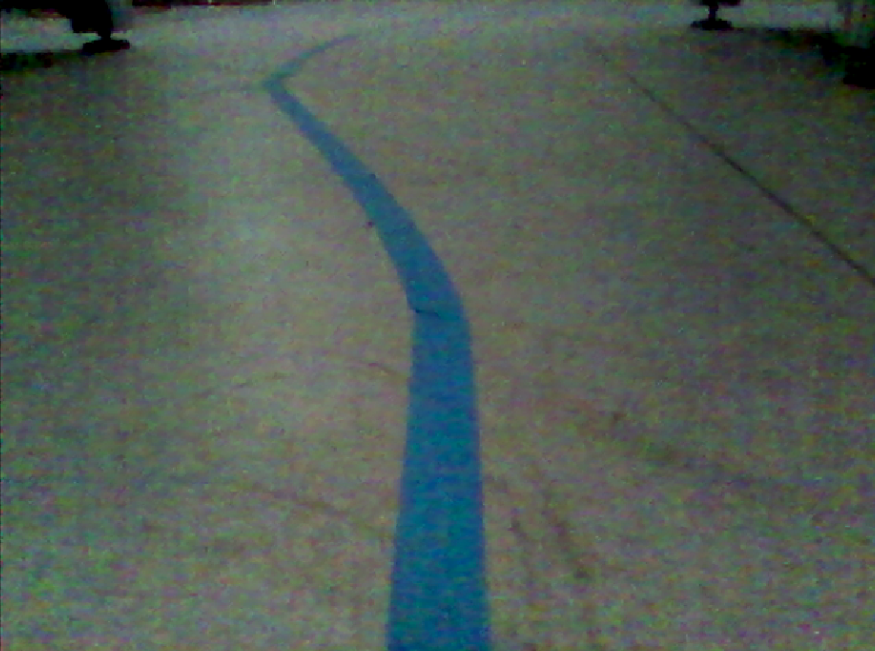
\includegraphics[width=\textwidth, height=7cm, keepaspectratio]{Bilder/line_unfilt_wenigLicht.png}
	\caption{Ungefilterte Aufnahme der Fahrlinie bei wenig Licht}
	\label{img:line_unfilt_wenigLicht}
	\end{figure}
\end{comment}


\paragraph{OneLineDetect}
Dieser Filter erhält das Binärbild und ermittelt die Position der blauen Linie relativ zur Position des Autos. Dafür wird in einer Bildzeile kurz unterhalb der Bildmitte (korreliert mit dem Bereich 20 cm vor dem Auto) nach der größten Anzahl weißer, zusammenhängender Pixel gesucht. Der Mittelpunkt wird berechnet und als Zentrum der dort verlaufenden Linie interpretiert. Der Abstand zwischen ermittelten Linienmittelpunkt und Bildmitte wird auf einen Wert zwischen -100 und 100 normiert und ausgegeben (siehe \autoref{graph:oneLineDet_reldotpos}).

\begin{figure}[h]
	\centering
	\begin{tikzpicture}[xscale=0.05,yscale=0.05]
	\draw[-] (-100,0) -- (100,0) node[right] {$Bildbreite$};
	\foreach \i in {-100, 0, 100}{
		\draw[-] (\i,-2) -- ( \i,2) node[above] {$\i$};
	}
	\draw[line width=1mm] (10,-2) -- (10,2) node[above right] {Bsp. Erkannte Linie};
	\end{tikzpicture}
	\caption{Beispiel eines errechneten Fahrstreifen-Mittelpunktes (bei 10) innerhalb einer Bildzeile, normiert auf den Bereich -100 bis 100}
	\label{graph:oneLineDet_reldotpos}
\end{figure}

Um die Berechnung der Linienmitte robuster zu gestalten, was besonders bei verrauschten Kamerabildern in dunklen Lichtverhältnissen nützlich ist, wird die Linienmitte auch in benachbarten Bildzeilen berechnet. Auf die errechneten Linienmittelpunkte wird der Median-Filter angewendet. Außerdem gibt es eine Mindestanzahl an zusammenhängenden weißen Pixeln, die erreicht werden muss, um als Fahrbahnmarkierung zu gelten.

Wird beispielsweise in einer Kurve in dem Bereich unter der Bildmitte keine Linie detektiert, so wird in einem zweiten Suchbereich nahe des unteren Bildrandes gesucht (siehe \autoref{img:line_filt_normal_u_kurve} (b)). Dieser Bereich korreliert mit dem Abstand von 5 cm vor dem Auto.

Wird auch hier keine Linie detektiert, wird der Wert -101 ausgegeben. 

Auf den Abbildungen \ref{img:line_filt_viel_u_wenig_licht} und \ref{img:line_filt_normal_u_kurve} sind in Rot jeweils diejenigen Punkte markiert, die zur Linienpositionierung erkannt wurden.


\begin{figure}
	\subfigure[Wenig gekrümmte Fahrstrecke]{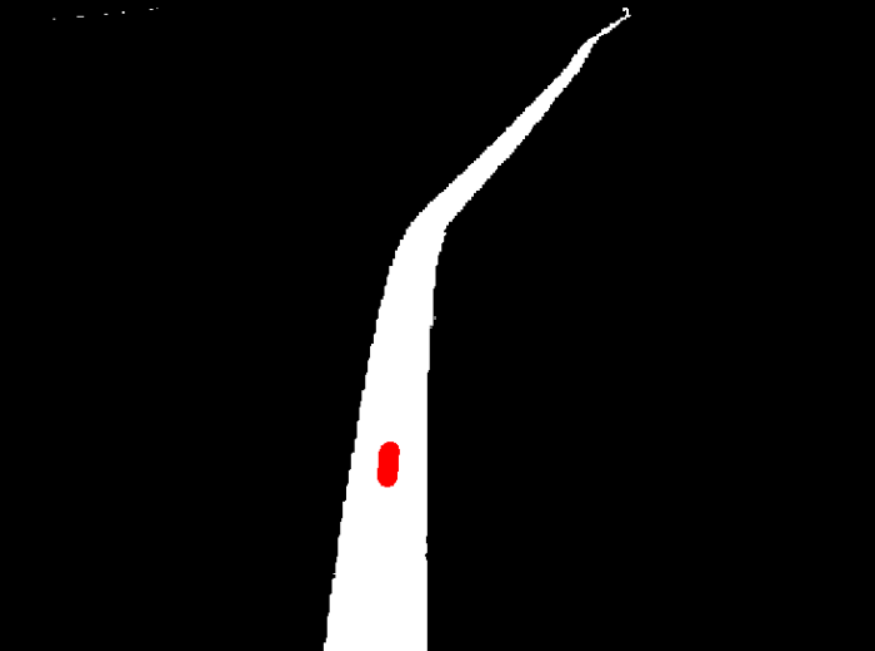
\includegraphics[width=0.49\textwidth]{Bilder/line_filt_normal.png}}
	\subfigure[Enge Kurve]{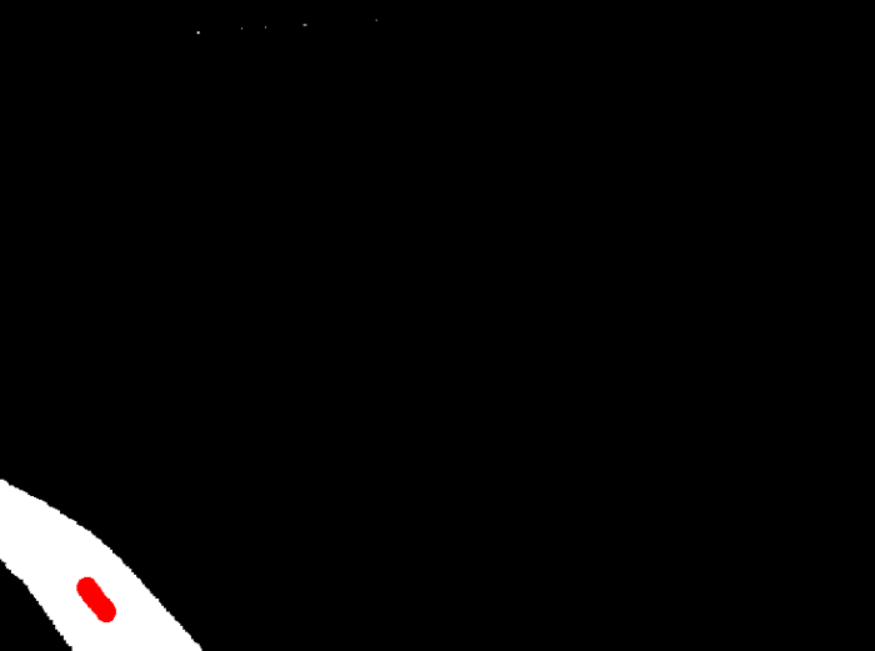
\includegraphics[width=0.49\textwidth]{Bilder/line_filt_engeKurve.png}}
	\caption{Gefilterte Linienerkennung unter normalen Lichtverhältnissen - unterschiedliche Behandlung gemäß Fahrbahnkrümmung}
	\label{img:line_filt_normal_u_kurve}
\end{figure}


\clearpage

\subsubsection{Abstandserkennung und -verwertung}
Die Abstandserskennung ist eine der grundlegenden Anforderungen an einen autonomen Roboter zur Ermöglichung von gefahrloser Navigation. In diesem Projekt wird sie auf Basis von Messwerten der zehn im Auto verbauten Ultraschallsensoren (siehe \autoref{img:car_ussensors})  implementiert.

Die eingehenden, mediangefilterten Abstandswerte liegen im Bereich von 0 bis 400 cm. Diese werden unterschiedlich gewichtet, dann der geringste Wert in eine Geschwindigkeit umgerechnet. Die Übersetzung eines Abstands- in einen Geschwindigkeitswert wird anhand einer linearen Funktion realisiert, die einen minimalen  Input-Grenzwert zum Anstoßen der Bewegung und gleichsam einen maximalen Input-Wert beinhaltet, ab dem die volle Geschwindigkeit zurück gegeben wird (siehe \autoref{graph:disttospeed}). Dies dient dazu, einen gewissen Mindestabstand beim Fahren nicht zu unterschreiten, sowie zum Ignorieren von Hindernissen, die weiter als ein gewisser Maximalwert von den Sensoren entfernt aufgefasst werden. Ersterer wird durch Testergebnisse statisch auf 20 cm gesetzt, letzterer auf 100 cm. Im Abstands-Wertebereich von 20 cm bis 100 cm gilt die lineare Funktion \emph{y = x}.

\begin{figure}[ht]
	\centering
	\begin{tikzpicture}[xscale=0.05,yscale=0.05,domain=0.125:220,samples=400]
	\draw[->] (-10,-10) -- (180,-10) node[below] {$Abstand (\centi\meter)$}; %x-Achse
	\draw[->] (0,-20) -- (0,115) node[left] {$Geschwindigkeit (Prozent)$}; %y-Achse
	\foreach \i in {20,40,...,150} { %x-Achsen-Schritte
		\draw (\i,-9) -- (\i,-11) node[below] {$\i$};
	}
	\foreach \i in {0,20,...,100} { %y-Achsen-Schritte
		\draw (1,\i) -- (-1,\i) node[left] {$\i$};
	}
	\draw[blue] (0,0) -- (20,0) ;
	\draw[blue, dotted] (20,0) -- (20,20);
	\draw[blue] (20,20) -- (100,100) -- (140, 100);
	\end{tikzpicture}
	\caption{Übersetzung von Abstandswert in prozentuale Geschwindigkeit}
	\label{graph:disttospeed}
\end{figure}

Die Geschwindigkeit wird mithilfe des kleinsten von allen Ultraschallsensoren gemessenen Abstandswertes berechnet. Da den zur Seite oder gar nach hinten gerichteten Sensoren bei geradliniger Fahrt nicht die selbe Priorität beigemessen werden sollte, wie den nach vorne ausgerichteten, wo der Abstand eher kollisionsrelevant ist, wird zunächst jeder Wert nach Relevanz gewichtet und entsprechend zu einem neuen Wert verrechnet. Mit jedem Sensor wird ein Winkel assoziiert, welcher auf den Bereich zwischen -1 und 1 abgebildet wird, wobei 0 die frontale Ausrichtung beschreibt. Der Bereich von 0 bis -1 beschreibt im Modell den gegen den Uhrzeigersinn gerichteten Halbkreis bis zum nach hinten gerichteten Sensor (\autoref{img:car_ussensors}; der Reihe nach die Sensoren (5), (4), (3), (2), (1), (0)) und äquivalent der von 0 bis 1 gehende Bereich den Halbkreis im Uhrzeigersinn zum nach hinten gerichteten Sensor  (\autoref{img:car_ussensors}; der Reihe nach die Sensoren (5), (6), (7), (8), (9), (0)). Alle rückgerichteten Sensoren werden der Einfachheit halber auf 1 respektive -1 abgebildet, da sie bei der normalen Fahrt nicht weiter von Interesse sind. Die Zuordnung der Winkel ist veranschaulicht in \autoref{img:car_ussensors}. 

\begin{figure}[ht]
	\centering
	\begin{tikzpicture}[xscale=3,yscale=3]
	\draw[->] (0,-1.1) -- (0,1.1);	%Pfeil
	
	%Zahlen auf dem Strahl
	\draw  (0.05,-1) -- (-0.05,-1) node[left] {$(-180\degree) -1$};
	\draw  (0.05,-0.7) -- (-0.05,-0.7) node[left] {$(-126\degree) -0.7$};
	\draw  (0.05,-0.4) -- (-0.05,-0.4) node[left] {$(-72\degree) -0.4$};
	\draw  (0.05,-0.2) -- (-0.05,-0.2) node[left] {$ (-36\degree) -0.2$};
	\draw  (0.05,-0) -- (-0.05,-0) node[left] {$(0\degree), +-0$};
	\draw  (0.05,0.2) -- (-0.05,0.2) node[left] {$(36\degree), +0.2$};
	\draw  (0.05,0.4) -- (-0.05,0.4) node[left] {$(72\degree), +0.4$};
	\draw  (0.05,0.7) -- (-0.05,0.7) node[left] {$(126\degree), +0.7$};	
	\draw  (0.05,1) -- (-0.05,1) node[left] {$(180\degree),+1$};

	%Sensoren
	\draw[-] (-0.05,1) -- (0.05,1) node[right]{$Rear Right(9)$};
	\draw[-] (-0.05,0.7)-- (0.05,0.7) node[right]{$SideRight(8)$};
	\draw[-] (-0.05,0.4) -- (0.05,0.4)  node[right] {$Front Right(7)$};
	\draw[-] (-0.05,0.2) -- (0.05,0.2)  node[right] {$Front Center Right(6)$};
	\draw[-] (-0.05,0) -- (0.05,0) node[right] {$Front Center(5)$};
	\draw[-] (-0.05,-0.2) -- (0.05,-0.2)  node[right] {$Front Center Left(4)$};
	\draw[-] (-0.05,-0.4) -- (0.05,-0.4)  node[right] {$Front Left(3)$};
	\draw[-] (-0.05,-0.7) -- (0.05,-0.7) node[right]{$SideLeft(2)$};
	\draw[-] (-0.05,-1) -- (0.05,-1) node[right]{$Rear Center(0);RearLeft(1)$};
	
	\end{tikzpicture}
	\caption{Ultraschallsensoren und ihr assoziierter Winkel, projiziert auf den Bereich zwischen -1 und 1}
	\label{graph:us-angles}
	
\end{figure}

Basierend auf diesen Winkeln wird gemäß einer Gauss-Kurve der Gewichtungsfaktor für den jeweiligen Sensor bestimmt, mit dem dessen Messwert multipliziert wird (dargestellt in \autoref{img:gaussian-weighted-dist-straight}). Dieser Faktor ist stets größer oder gleich 1, was bedeutet, dass ein gemessener Abstand nur zunehmen und damit an Relevanz verlieren kann, wenn es darum geht, im Anschluss den kleinsten zur Geschwindigkeits-Berechnung zu wählen.

\begin{figure}[!ht]
	\centering
	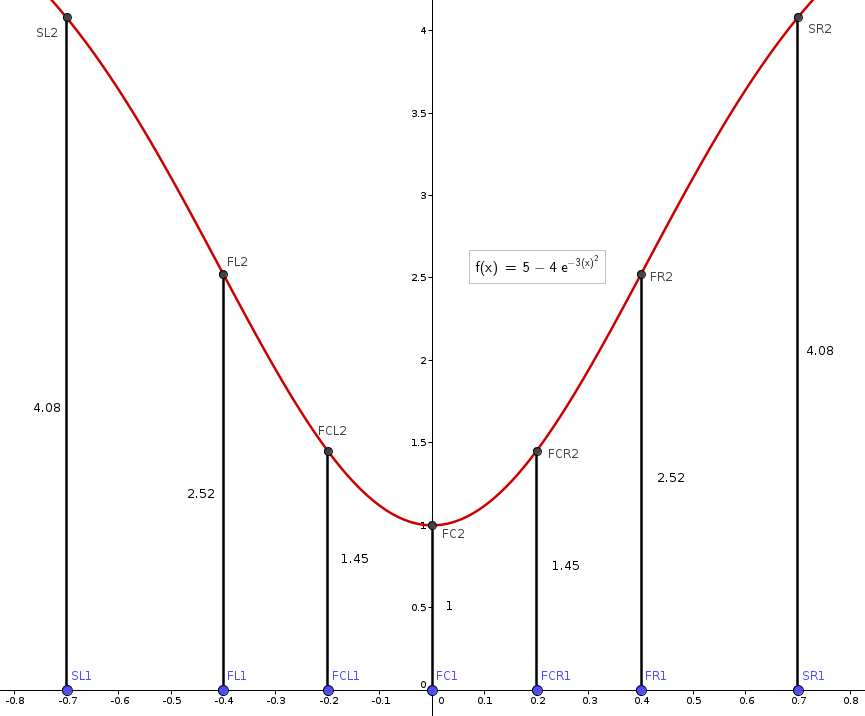
\includegraphics[width=\textwidth, height=11cm, keepaspectratio]{Bilder/Gauss_Sensorgewichtung_gerade.png}
	\caption{Gewichtung der Abstands-Messwerte beim Geradeaus-Fahren}
	\label{img:gaussian-weighted-dist-straight}
\end{figure}

\begin{figure}[!ht]
	\centering
	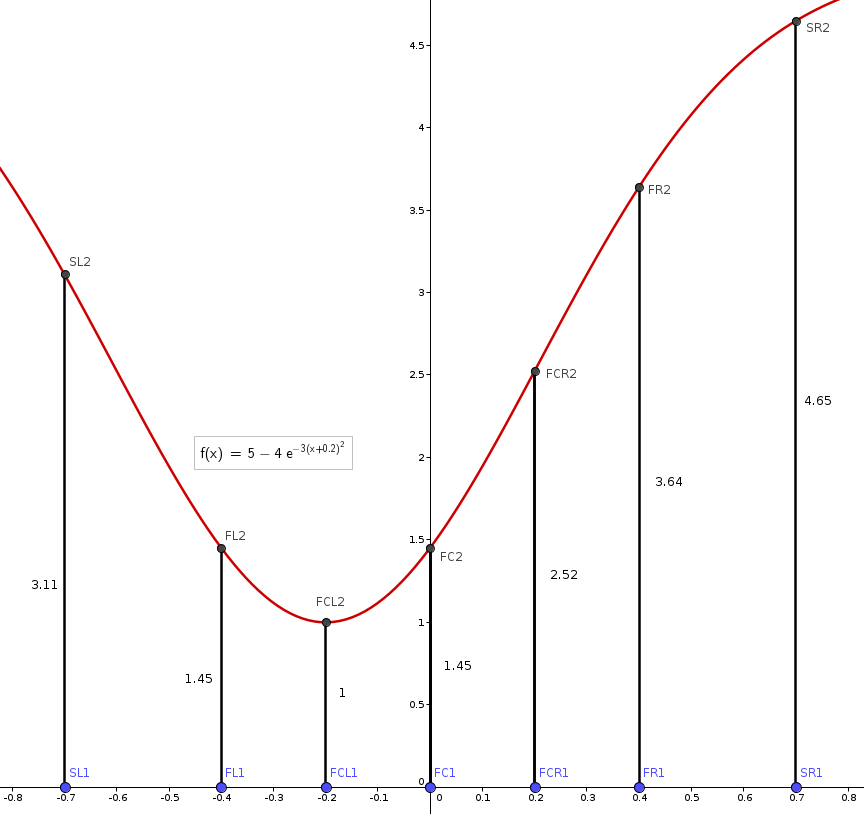
\includegraphics[width=\textwidth, height=12cm, keepaspectratio]{Bilder/Gauss_Sensorgewichtung_geneigt.png}
	\caption{Gewichtung der Abstands-Messwerte bei Lenkung nach links (maximale Verschiebung)}
	\label{img:gaussian-weighted-dist-curve}
\end{figure}

Solche statisch festgelegten Gewichtungsfaktoren sind aber vor allem für ein Geradeaus-Fahren mit gewisser Geschwindigkeit optimiert. Das ist beispielsweise in Kurven problematisch, in welchen das Hauptaugenmerk nicht mehr geradeaus liegen sollte, da die Geschwindigkeit durch links oder rechts vorbeifahrend frontal erkannte Hindernisse unnötig gedrosselt werden würde. Daher wird eine dynamische Anpassung des relevanten Sensor-Blickkegels realisiert. Dazu wird gemäß des eingeschlagenen Lenkwinkels, der dazu auf den Bereich von -1 bis 1 normiert einfließt, die Gauss-Kurve auf der x-Achse verschoben, wie dargestellt in \autoref{img:gaussian-weighted-dist-curve}.

Konkret sind in \autoref{img:gaussian-weighted-dist-straight} und \ref{img:gaussian-weighted-dist-curve} die fixen Ablesepunkte der einzelnen Sensoren auf der x-Achse abgebildet, welche an den Sensor-Winkeln in Blickrichtung des Autos angelehnt werden. Der entsprechende Punkt auf der Gauss-Kurve gibt den jeweiligen Gewichtungs-Faktor an, wobei ein größerer Wert eine größere Unempfindlichkeit bedeutet. Gemäß Lenkwinkel wird nun die Kurve auf der x-Achse verschoben, wodurch die Gewichtung sich auf die entsprechend seitlich liegenden Sensoren verschiebt.

Die Gauss-Kurve entspricht folgender Formel,

\begin{equation}\label{eq:gaussian-weighted-dist}
sensorWeight= 5 - 4 * \exp\Bigl({-3 * (sensorAngle - steeringAngle)^2}\Bigr)
\end{equation}
wobei $sensorAngle$ der auf den Bereich zwischen -1 und 1 normierte Sensorwinkel ist, für den eine Gewichtung berechnet werden soll, und $steeringAngle$ der eingeschlagene Lenkwinkel, ebenfalls im Bereich zwischen -1 und 1 liegend. Die Höhe der Kurve, bestimmt durch die addierte 5 sowie die multiplizierte -4, wurden durch Versuche als angemessen herausgestellt und festgelegt.

\clearpage

\subsubsection{Motoransteuerung}
Die zentrale Aufgabe der Motoransteuerung ist die Aufbereitung und Weitersendung der Geschwindigkeit und des Lenkwinkels an die Aktoren sowie die Initialisierung des Speed Controllers.

Da die interne Kommunikation der Motordaten auf Werte zwischen -100 bis 100 normiert sind, ist eine Umrechnung dieser in reale Steuerdaten notwendig. Hierbei lässt sich auch die Maximalgeschwindigkeit festlegen bzw. drosseln. Bedingt durch Reaktionszeiten der Sensoren hat sich eine Drosselung auf 12 Prozent der tatsächlichen Maximalgeschwindigkeit bewährt.

Um zeitkritisch auf ein von den Ultraschallsensoren detektiertes Hindernis mit einem Nothalt reagieren zu können, empfängt die Motorensteuerung Flags direkt von der Ultraschallauswertung und umgeht damit weitere Programmlogik.
   

\subsection{Interprozesskommunikation}

Da die Programmierung in verschiedenen Funktionsblöcken erfolgte, musste eine einheitliche Kommunikation sichergestellt werden. Hierzu wurde eine separate Funktionssammlung erstellt, die von allen Funktionsblöcken inkludiert wurde. Sie beinhaltet Definitionen über den Nachrichtentyp und die Zusammensetzung strukturierter Datentypen. Da der vom ADTF gestellte Ablauf zum Senden oder Empfangen eines bestimmten Nachrichtentyps zur Codeverdopplung in den Funktionsblöcken führen würde, wurden die Funktionen zusammengefasst und ausgelagert. Damit ließ sich auch einheitlich sicherstellen, dass Funktionsblöcke beim Empfangen die Nachricht erst Kopierten, bevor deren Inhalt verändert wurde.

\subsection{Projektstruktur}
Die drei zuvor beschriebenen Aufgabenbereiche werden über ADTF in Funktionsblöcke aufgeteilt.



\begin{figure}[ht]
	\centering
	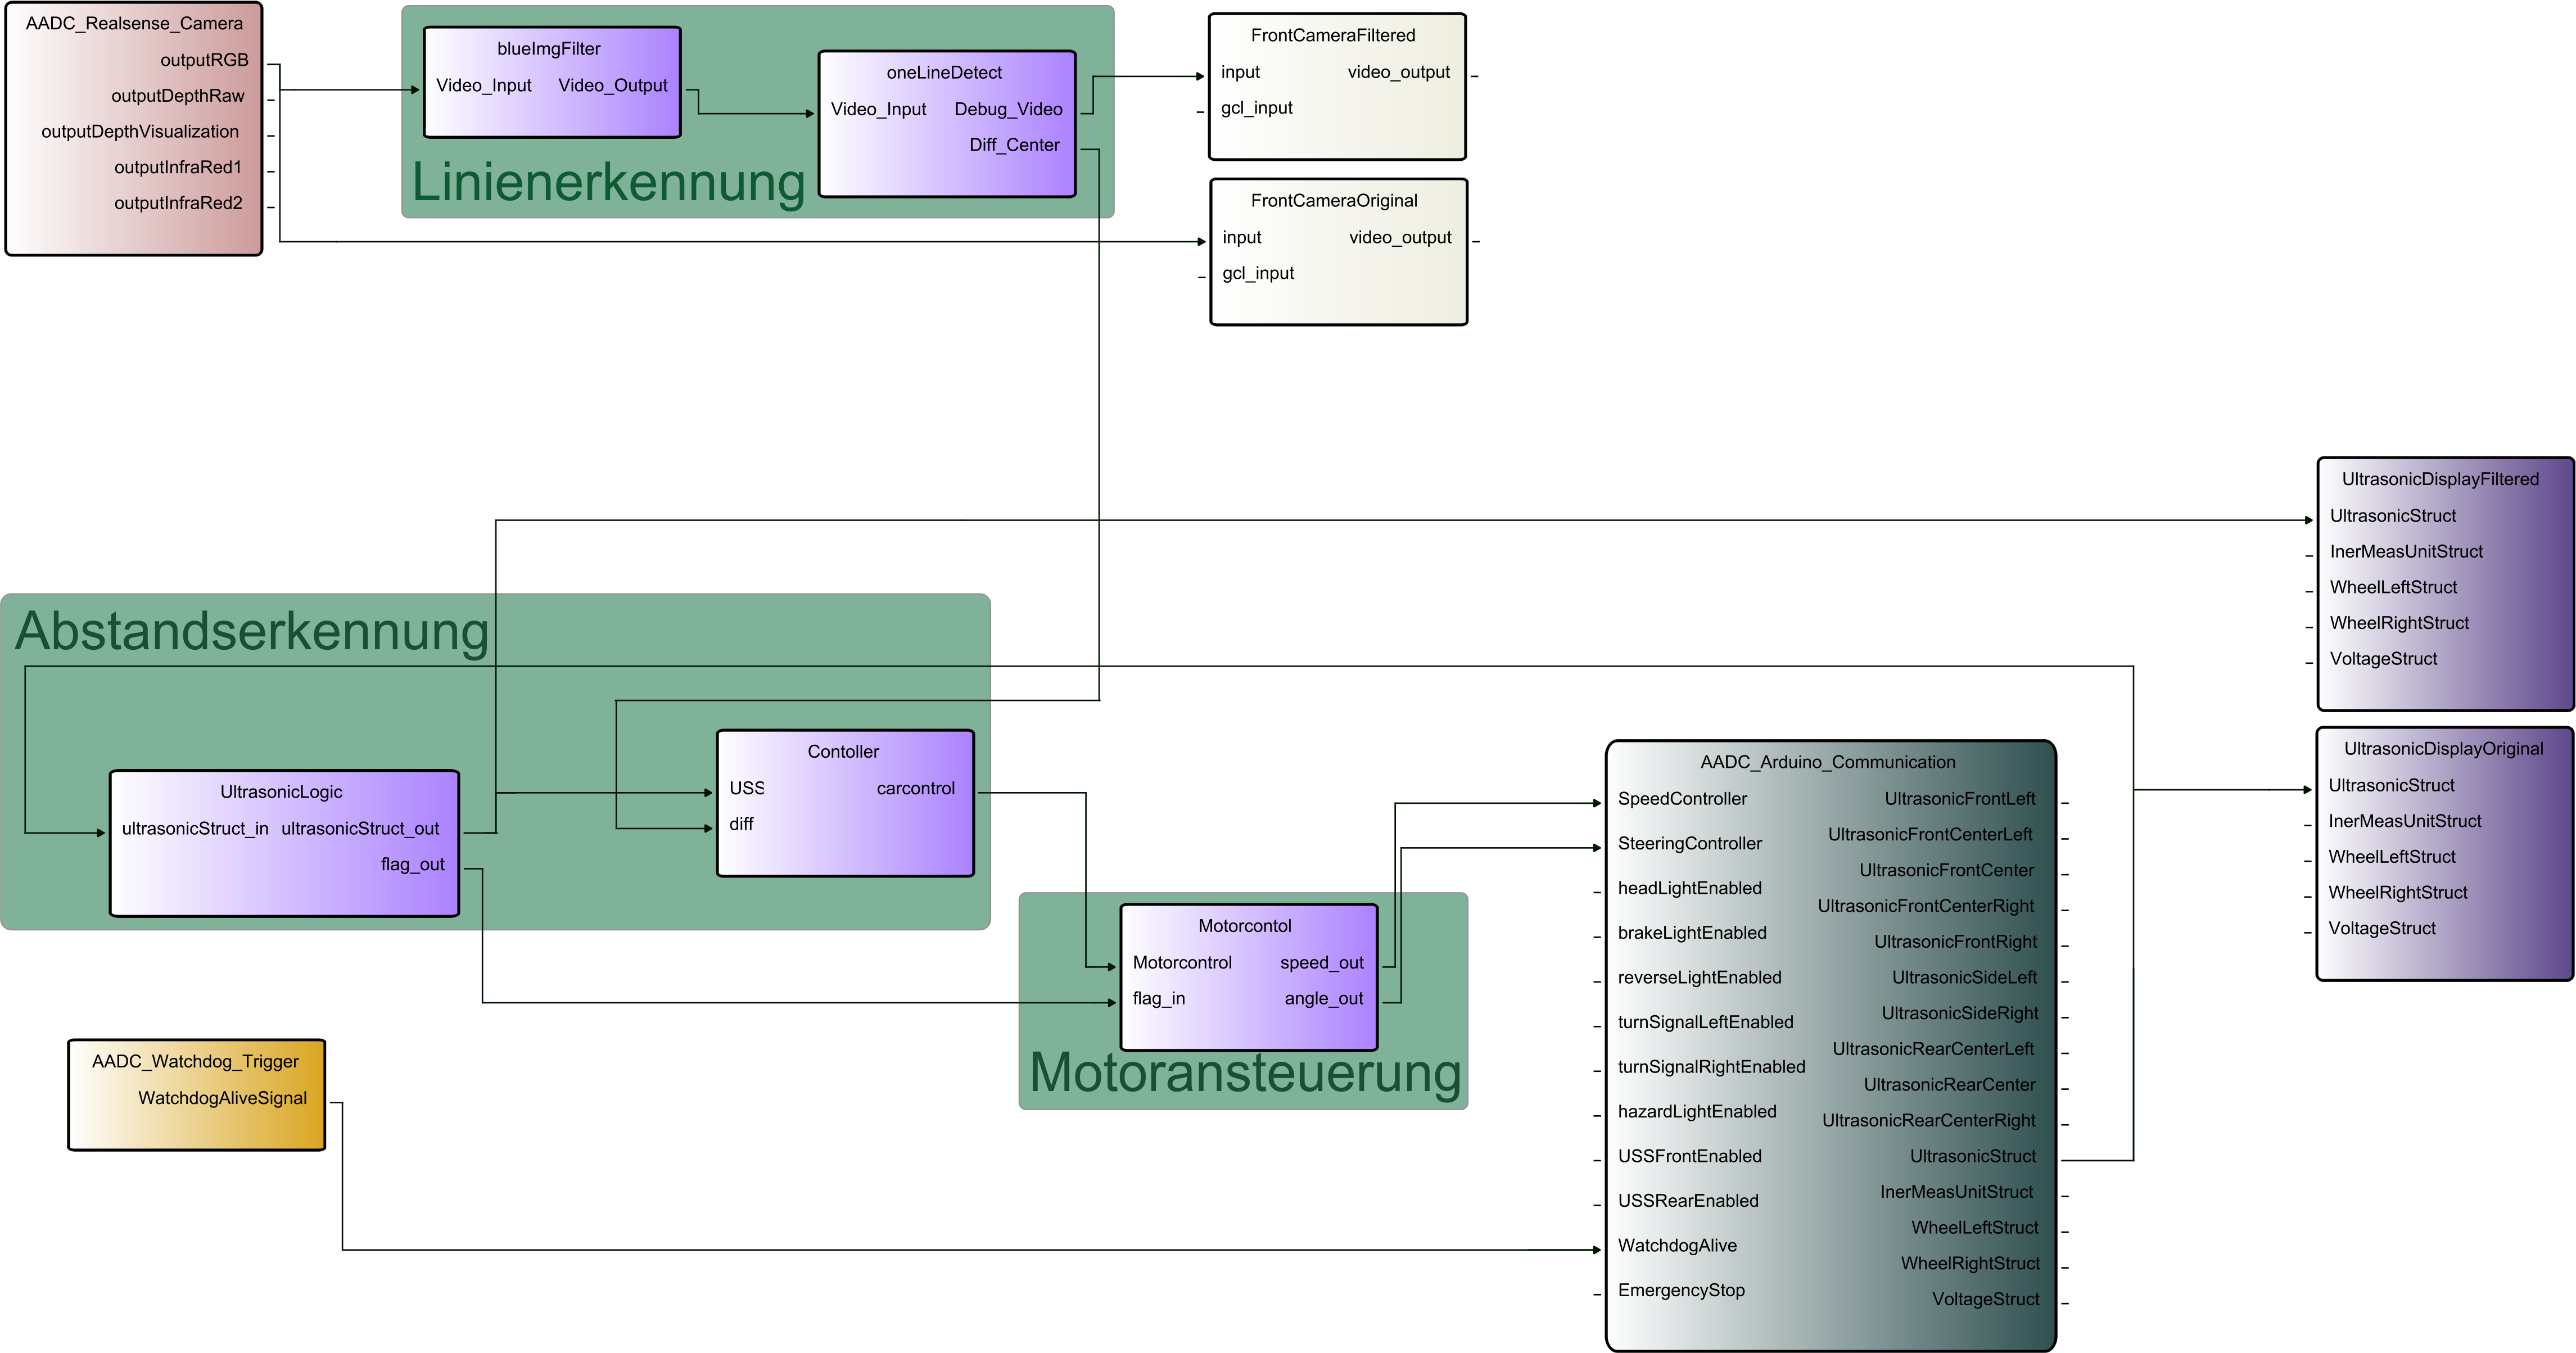
\includegraphics[width=\textwidth, height=\textheight, keepaspectratio]{Bilder/FunktionsblockplanE.png}
	\caption{Funktionsblockplan der Test-Umgebung}
	\label{img:funktionsblockplan}
\end{figure}


\subsection{Komplikationen und Fehler}
Im Folgenden findet sich eine Auflistung von Fehlern und Komplikationen, die während der Entwicklung auftraten und zu Einschränkungen, der in der Roadmap gesetzten Ziele führen.

\subsubsection{ADTF}
\paragraph{Dokumentation}
Der Umgang mit dem ADTF gestaltet sich zu Anfang sperrig. Zu vielen vorgefertigten Filtern fehlt die Schnittstellenbeschreibung. Auch die im Projekt genutzte Kommunikation zwischen den Filtern ist nicht einheitlich und lässt sich daher nur mühsam verstehen. So ist die Kommunikation mit dem Arduino-Filter mittels einer Sequenzialisierung und der Übermittlung des Signals in Klarschrift eine gänzlich andere, als die Weitergabe von Zeigern auf Speicherbereiche, wie an anderer Stelle verwendet.

\paragraph{Nutzung in virtueller Maschine}
Die parallele Filterentwicklung setzt das verwenden von virtuellen Maschinen voraus, doch von ADTF bereitgestellte Funktionen zur grafischen Darstellung von Videosignalen funktionieren damit nicht. Hierfür ist ein weiterer im Nachhinein selbst implementierter Filter erforderlich.

\subsubsection{Kalman-Filter}
Zur Filterung von Messwerten wird ein Median-Filter mit jeweils parametrisierter Länge verwendet, anstelle eines ursprünglich in der Roadmap geplanten Kalman-Filters. Grund dafür ist, dass die Implementierung der in der Roadmap beschriebenen Funktionen eine einheitliche Kommunikation voraussetzt. Die dort entstandene Entwicklungszeit wird durch den weniger aufwendigeren Median-Filter kompensiert.

\subsubsection{Ultraschallsensoren}
Da die Ultraschallsensoren über das ADTF zu schnell abgefragt werden, kann ein Sensor das Echo eines anderen Sensors detektieren und damit eine falsche Abstandmessung ausgeben. Solche Fehlmessungen können dazu führen, dass das Auto während der Fahrt ohne augenscheinlich erkennbaren Grund seine Geschwindigkeit verringert, da vermeintliche Hindernisse erkannt werden.

\subsubsection{Beschleunigungssensor}
Die Verwendung des Beschleunigungssensors setzt einen angepassten Kalman-Filter voraus, da bereits Vibrationen des Motors ausreißende Messwerte von bis zu 2 G erzeugen. Deshalb ließ sich die geplante Funktion, Stoppen des Motors bei anheben des Fahrzeugs, nicht ohne weiteres realisieren. 

\newpage
%%% Neues Kapitel %%%
\section{Auswertung}
Das Auto folgt, wie in der Zielsetzung beschreiben, einer blauen Linie und passt seine Geschwindigkeit erkannten Hindernissen bist zum Halt in gegebenem Mindestabstand an.

Der Einsatz eines Median-Filters anstatt eines Kalman-Filters führt zu keinen Einschränkungen.

Die Linienerkennung ist einfach implementiert und ist deshalb nur unter eng gefassten Rahmenbedingungen nutzbar. Zusätzliche blaue Farbbereiche im relevanten Sichtfeld werden eventuell als Fahrbahnmarkierung interpretiert.

Durch die erstmalige Verwendung des Modells zu Lehrzwecken, ist zu wenig über die genaue Funktionsweise aller gegebener Funktionen bekannt. Deshalb floss zu viel Arbeitszeit in die Einarbeitung und Auseinandersetzung mit ADTF, anstelle von eigentlicher Filterimplementierung.

\section{Ausblick}
Das Projekt bietet viel Potenzial für Erweiterungen.

Im Baustein \emph{OneLineDetect} beispielsweise wurde bereits eine zweite Funktion implementiert, die es ermöglicht, die zwei breitesten Linienquerschnitte in einer Bildzeile zu ermitteln und direkt eine entsprechende Entscheidung zu treffen, welche weiter verarbeitet werden soll. Nach Anpassung der globalen Schnittstellen könnten später bei Erkennung mehrerer Linien diese weiter gereicht und vom zentralen Logik-Baustein entsprechend im Sinne einer Abbiege-Entscheidung verwertet werden.

Auch die Gewichtung der gemessenen Ultraschall-Abstandsmesswerte könnte im nächsten Schritt nicht nur, wie bislang, gemäß eingeschlagenem Lenkwinkel im Sinne einer seitlichen Relevanzverschiebung angepasst werden, sondern auch entsprechend der aktuellen Geschwindigkeit generell mehr oder weniger empfindlich gemacht werden (dynamisches Stauchen/ Strecken der Gauss-Kurve).

Es bleibt zu hoffen, dass die anfänglich investierte Zeit des Aufsetzens der und Einarbeitens in die Umgebung weitere Arbeit an ähnlichen Projekten problemorientierter und -fokussierter ermöglichen kann.


\newpage
\addcontentsline{toc}{section}{Abbildungsverzeichnis}
\listoffigures

\end{document}
